\begin{abstract}
This chapter is the first study to reveal the dynamics of time-varying oligopsonistic competition and storage adoption, and their impact on smallholder farmers' welfare. While existing research explores storage incentives like risk preferences and trading costs, it overlooks the advantages of quality-preserving technologies for accessing time-varying competitive markets. Cold storage adoption, especially for perishable crops, helps farmers overcome trading-time limitations. By constructing a two-period post-harvest management model for a storable cash crop, I find that temporal changes in trader competition alone suffice for farmers to benefit from storage. This work has broader relevance to settings with multiple input suppliers selling to a limited set of traders involved in market division and price fixing over time.


\keywords{Storage Adoption, Time-varying Oligopsony, Farmer Welfare}

\end{abstract}

%--------------------------------------------------------%
\section{Introduction}
\noindent    Buyer power arises from the immobility of certain factor inputs that, in the short run, are largely “captive” to a limited set of buyers. While spatial immobility has been extensively explored in the literature, the impact of changes in temporal immobility on bargaining dynamics remains underexamined. This gap is particularly relevant in agricultural markets, where products are typically perishable, and storage plays a critical role in the supply chain.

Smallholder farmers in developing countries often contend with the oligopsony power of middlemen and processors \footnote{In this study, the terms middlemen, field buyers, intermediaries, and traders will be used interchangeably to refer to a group of buyers who directly purchase fresh apples from farmers. These buyers play a crucial role in the supply chain by acting as the initial link between farmers and the broader market. They typically visit orchards, negotiate prices with farmers, and handle the immediate procurement of apples. Their role may also include transporting apples to wholesale markets, processing units, or exporters, depending on the supply chain dynamics. Regardless of the specific term used, all these buyers share the common function of directly sourcing apples from farmers before the produce reaches larger market players, such as wholesalers, retailers, or processors.}, leading to substantial margins for the latter \citep{rogers_rich_1994assessing}. While existing literature primarily explores the correlation between market power and "spatial" trading frictions such as transportation and price-search costs \citep{bergquist_dinerstein_2020,mitra_mookherjee_torero_visaria_2018,ranjan_2017,antras_costinot_2011}, the reasons behind small farmers frequently missing out on inter-temporal marketing opportunities remain a subject of controversy \citep{williams1991storage, wright1984welfare, ruhinduka2020smallholder, lai2003optimal}.

Facing time-sensitive post-harvest decisions, small-scale farmers must choose between immediate and delayed selling, with limited access to quality-preserving technologies like cold storage constraining their marketing window \citep{aggarwal2018grain}. Despite some developing countries offering partial storage subsidies, the inherent variability in agricultural prices and the fixed cost of initial storage construction often make storage adoption a challenging investment for smallholder farmers, particularly in cash crops.

In reality, predicting storage returns proves challenging for farmers, and the volatility in farm-gate prices can discourage them from storing crops for future sales, even with access to credit \citep{cardell2023price}. Previous literature emphasizes the pivotal role of factors such as storage costs, downstream supply and demand shocks, perishability of produce, and risk aversion in influencing farmers' post-harvest decisions and welfare consequences. However, the potential competitive advantages of storage, enabling farmers to enter more competitive procurement-market conditions, have received limited exploration in the existing literature.

To the best of our knowledge, this study is the first to unveil the interplay of farmers' (sellers') storage adoption with time-varying procurement market conditions. Without the adoption of storage, farmers who cultivate crops that spoil quickly face limitations in their trading options, as they can only sell their produce locally at harvest time, because smallholder farmers usually lack access to trucks which prevents them from accessing distant selling locations. But if they are equipped with advanced storage technology, they would be able to seek out a higher local price brought from more competitive market conditions among middlemen in the later periods as shown in Figure \ref{Figure: Demo}.

\begin{figure}[ht]
\centering
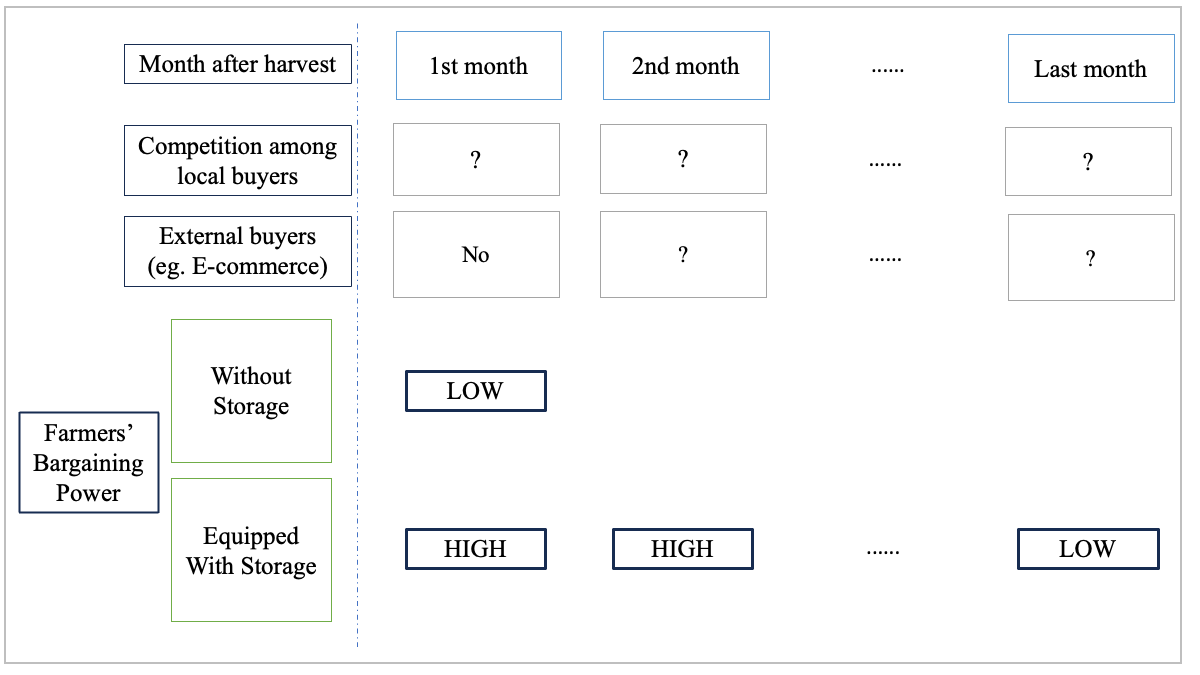
\includegraphics[width=1\textwidth]{figures/graphic_demo.png}
\caption{Extended Marketing Opportunities from Storage Adoption}
\label{Figure: Demo}
\end{figure}

Specifically, farmers could potentially benefit from increased competition in the oligopsonistic market through two sources. Firstly, the presence of different intermediaries in the village at various times can create fluctuating levels of competition on a monthly or even weekly basis. Traders may perceive villages with greater storage as having a lower instantaneous supply of storable goods due to a smaller fraction of farmers being forced to sell. This perception leads traders to be willing to offer higher prices in these villages to secure the available supply. This allows farmers with storage options to sell their produce at the most advantageous time. Secondly, farmers with storage can tap into additional distribution channels such as e-commerce and direct selling, which differ from the conventional middlemen-dominated system. By doing so, they can introduce external participants into the oligopsonistic market at the farm gate at different time nodes. 

I develop a conceptual framework to explore how smallholder farmers adopt cold storage to bargain against the time-varying buyer power of middlemen. It considers a simplified dynamic two-period scenario in a developing country, where farmers sell a specific cash crop to middlemen due to high transaction costs associated with accessing larger markets. The model incorporates a storage-decision process, wherein farmers, observing farm-gate prices at harvest, decide whether to sell or store their crops.

The outcomes of this study hold substantial implications for policymakers and farmers alike. By exploring the dynamics of time-varying oligopsony levels, the research aims to demonstrate the potential benefits of storage facilities for both producers and consumers. In a broader context, the findings suggest that embracing storage adoption could provide farmers with an effective alternative to combat anticompetitive practices like market division and avoid more intrusive measures in markets, such as governments fixing prices.





\section{Base Model}
\noindent  I propose a two-period dynamic model examining how smallholder farmers strategically adopt storage in response to middlemen's time-varying buyer power. The setting is a rural region in a developing country, where smallholder farmers primarily rely on selling a cash crop to middlemen due to prohibitively high transaction costs associated with accessing distant markets. I treat the harvest quantity as exogenous and focus on farmers' storage and marketing decisions within a single crop year.

Farmers are assumed to exhibit risk preferences ranging from risk neutrality to moderate risk aversion, valuing their own consumption at prevailing market prices. Their decision problem centers on choosing the optimal share of the harvest, $s \in [0,1]$, to store immediately after harvest. This choice is made under uncertainty about future market conditions, specifically the evolution of buyer power in the subsequent trading period.

In the first trading period, farmers observe farm-gate price offers from middlemen. Price heterogeneity, stemming from quality differences, is aggregated into a single representative price for tractability. Farmers infer the degree of contemporaneous buyer power ($\theta_1$) based on the number of offers and local information-sharing, understanding that greater buyer competition (lower $\theta_1$) is associated with higher farm-gate prices ($p_1$). Assuming the relationship between buyer power and prices persists across periods, farmers then decide the portion of the harvest to sell immediately and the portion to store, anticipating potential changes in middlemen competition (thus in $\theta_2$).  

I assume symmetric information and zero transaction costs in each trading period. Thus, farmers can fully realize the prevailing farm-gate prices at the time they sell.

Formally, the farming household's objective is to maximize expected discounted utility over the two trading periods, choosing $s$ given harvest quantity $q=1$\footnote{The harvest quantity $q$ is normalized to 1 for simplicity.}, as follows:
\begin{equation}
\label{eq:starting objective}
    \max_{s \in [0,1]} \left[ U\left((1-s) p_1\right) + \delta \mathbb{E}_a\left[ U\left(s \tilde{p}_2\right) \right] \right],
\end{equation}
where the first term captures utility from first-period sales, the second term captures expected utility from second-period sales, and $\delta \in (0,1]$ denotes a discount factor reflecting storage costs and potential present-biased preferences.

\subsection{Farmer Risk Preferences}
\noindent Farmers' preferences are modeled using a Constant Relative Risk Aversion (CRRA) utility function:
\begin{equation}
U(x) = \frac{x^{1-\gamma}}{1-\gamma},  \quad 0 \leq \gamma < 1
\label{eq: CRRA}
\end{equation}
where $\gamma$ denotes the degree of relative risk aversion.

The choice of CRRA utility is motivated by two factors. First, empirical evidence indicates that individuals’ relative risk aversion is approximately constant across different wealth levels \citep{chiappori2011relative}. Second, the unitless CRRA coefficient enables meaningful cross-context and international comparisons of risk preferences \citep{hardaker2000some}. This functional form also aligns with empirical findings from regions close to my fieldwork sites. For example, \citet{jin2024losses} document consistent risk-averse behaviors among apple growers in areas overlapping substantially with my study regions.

\subsection{Middlemen Market Structure and Farm-Gate Price Formation} \label{Section: Middlemen Market Structure and Farm-Gate Price Formation}
\noindent Given the model's focus on farmers' strategic use of storage as a bargaining mechanism, it is critical to embed a price formation structure that flexibly accounts for different degrees of middlemen competition.  

I employ the Flexible Oligopoly/Oligopsony Market (FOOM) framework to model farm-gate pricing as a function of buyer power. Assuming perfect competition in the downstream retail market, the farm-gate price $p_f$ is:
\begin{equation}
p_f = \frac{p_r - c}{1 + \frac{\theta}{\varepsilon}},
\end{equation}
where $p_r$ is the downstream retail price, $c$ denotes the buyers' constant marginal cost, $\theta$ captures buyer-side market power, and $\varepsilon$ is the farm supply elasticity facing buyers.

Normalizing the downstream price net of marginal costs to 1, $p_r - c = 1$, the farm-gate price simplifies to:
\begin{equation}
p_f = \frac{\varepsilon}{\varepsilon + \theta}.
\end{equation}

Given that the harvest is essentially fixed at the time of decision-making, but sales timing remains elastic, I assume $\varepsilon = 1$ as a plausible baseline. Thus, farm-gate prices reduce further to:
\begin{equation}
p_f = \frac{1}{1+\theta}, \quad \theta \in [0,1],
\label{Eq: price formation by buyer power}
\end{equation}
where $\theta=0$ corresponds to perfect buyer competition, $\theta=1$ reflects monopsonistic conditions, and intermediate values capture varying degrees of oligopsony power.

Assuming farmers believe that this price formation rule persists across periods, period-specific prices are determined as $p_t = \frac{1}{1+\theta_t}, \quad t=1,2$. At harvest time, farmers observe $p_1$ and infer the contemporaneous buyer power, $\theta_1 = \frac{1 - p_1}{p_1}$. They then form expectations about the evolution of buyer power between periods:
\begin{equation}
\theta_2 = \theta_1 + a,
\end{equation}
where $a$ is a stochastic shift capturing intertemporal changes in buyer competition.  
Thus, conditional on $a$, the second-period price is:
\begin{equation}
p_2(a) = \frac{p_1}{1 + a p_1}.
\label{Eq: p_2 of buyer power change}
\end{equation}

\subsection{Final Objective Function}

\noindent The economic environment faced by the farmer at the time of harvest is summarized in Table~\ref{tab:baseline model parameter table}. This includes both observed and unobserved elements that affect the storage decision over two periods.

\begin{table}[H]
\centering
\caption{Economic Environment at Harvest}
\label{tab:baseline model parameter table}
\begin{tabular}{lll}
\toprule
\textbf{Item} & \textbf{Symbol (units)} & \textbf{Status at Harvest} \\
\midrule
Harvest quantity & $q$ & Known, fixed (normalized to 1) \\
First-period price & $p_1$ & \textbf{Observed} \\
Inferred buyer power & $\theta_1 = \frac{1 - p_1}{p_1}$ & \textbf{Unobserved}, inferred from $p_1$ \\
Buyer-power change & $a$ & \textbf{Random} \\
Second-period buyer power & $\theta_2 = \theta_1 + a$ & Unknown \\
Price formation & $p_t = \frac{1}{1 + \theta_t},\ t=1,2$ & Derived \\
Discount factor & $\delta \in (0,1]$ & Observed \\
CRRA risk aversion & $0 \leq \gamma < 1$ & Observed \\
\bottomrule
\end{tabular}
\end{table}

\noindent Substituting the CRRA utility specification (Equation~\ref{eq: CRRA}) and the price formation rule (Equation~\ref{Eq: p_2 of buyer power change}) into the base objective function (Equation~\ref{eq:starting objective}), I obtain the final expression for the farmer’s intertemporal optimization problem:
\begin{equation}
\label{eq:final_objective}
\max_{s \in [0,1]} \frac{1}{1-\gamma} \left[ (1-s)^{1-\gamma} p_1^{1-\gamma} + \delta\, s^{1-\gamma} p_1^{1-\gamma} \mathbb{E}_a\left( (1 + a p_1)^{\gamma-1} \right)\right].
\end{equation}
\noindent The expression inside the expectation, $\mathbb{E}_a[(1 + a p_1)^{\gamma - 1}]$, represents the anticipated relative gain from deferring sale, focusing on uncertainty in future buyer power.

\subsection{Analytical Solutions}

\subsubsection{Risk-Averse Farmers}

\noindent To derive the optimal storage share for risk-averse agents ($0 < \gamma < 1$), I solve the first-order Kuhn–Tucker condition associated with the objective function in Equation~\ref{eq:final_objective}. For interior solutions where $0 < s < 1$, the necessary condition for optimality becomes:
\begin{equation}
    -(1 - s)^{-\gamma}(q p_1)^{1 - \gamma} + \delta s^{-\gamma}(q p_1)^{1 - \gamma} \mathbb{E}_a\left( (1 + a p_1)^{\gamma-1} \right) = 0.
\end{equation}
\noindent Simplifying, I obtain the optimal storage share:
\begin{equation}
\label{eq:s_star}
s^*(p_1, \delta, \gamma, a) = \frac{\left[\delta\, \mathbb{E}_a\left( (1 + a p_1)^{\gamma - 1} \right)\right]^{1/\gamma}}{1 + \left[\delta\, \mathbb{E}_a\left( (1 + a p_1)^{\gamma - 1} \right)\right]^{1/\gamma}}.
\end{equation}

This formulation highlights the dependency of the optimal decision on four key inputs: the first-period price ($p_1$), the intertemporal discount factor ($\delta$), the agent’s risk aversion parameter ($\gamma$), and the stochastic evolution of buyer power (via $a$). The expression captures a convex trade-off between immediate certainty and delayed, risk-adjusted returns.

Strict corner solutions ($s^* = 0$ or $s^* = 1$) are rare in this framework due to the continuous nature of CRRA utility. Notably, $s^* = 0$ arises only when the marginal utility of delayed sale is strictly less than that of immediate sale, i.e., when $\left[\delta\, \mathbb{E}_a\left( (1 + a p_1)^{\gamma - 1} \right)\right]^{1/\gamma} \leq 0$. However, since utility becomes unbounded as consumption approaches zero, a solution of $s^* = 1$ is not permissible when $\gamma > 0$.

In practical terms, solutions near the boundaries of the decision space occur frequently. For instance, I define *near-zero storage* as $s^* < 0.05$ and *near-full storage* as $s^* > 0.95$. These threshold cases arise under various plausible configurations of $p_1$, $\delta$, and the distribution of $a$, and are observed regularly in simulation results.

\subsubsection{Risk-Neutral Farmers}

\noindent When $\gamma = 0$, the farmer becomes risk neutral, and the utility function reduces to a linear form:
\[
U(x) = x.
\]
\noindent The problem thus simplifies to maximizing expected monetary value:
\[
\max_{0 \leq s \leq 1} \left[ (1-s) p_1 + \delta \, s \, \mathbb{E}_{a}\left( \frac{p_1}{1 + a p_1} \right) \right].
\]
\noindent Given that $q p_1 > 0$ and the harvest is normalized to 1, this reduces to:
\[
\max_{0 \leq s \leq 1} \left[ (1-s) + \delta\, s \, \mathbb{E}_a\left( \frac{1}{1 + a p_1} \right) \right].
\]
\noindent The corresponding first-order condition (FOC) is:
\[
\delta \, \mathbb{E}_a\left( \frac{1}{1 + a p_1} \right) = 1.
\]

\noindent The solution to this condition implies a threshold policy:
\begin{equation}
s^*(\gamma = 0) = 
\begin{cases}
1, & \delta \cdot \mathbb{E}_a\left[\frac{1}{1 + a p_1}\right] > 1 \\
0, & \delta \cdot \mathbb{E}_a\left[\frac{1}{1 + a p_1}\right] < 1 \\
\text{any in } [0,1], & \text{if equality holds}
\end{cases}.
\end{equation}

Under risk neutrality, the farmer evaluates only the expected monetary payoff. The decision thus reduces to a binary choice based on whether the discounted expected second-period price exceeds the normalized current price. If $\delta \, \mathbb{E}_{a}\left( \frac{1}{1 + a p_1} \right) > 1$, storage yields a higher expected return, and the farmer stores the entire harvest. If the inequality is reversed, the entire harvest is sold immediately. Indifference over any $s \in [0,1]$ occurs precisely when the two expected payoffs are equal.

This decision rule underscores the stark difference between risk-neutral and risk-averse behavior. Whereas risk-averse farmers smooth consumption across periods to mitigate uncertainty, risk-neutral farmers purely optimize expected return, disregarding variability in outcomes.




\subsection{Comparative Statics}

\noindent In this section, I investigate how changes in key model parameters influence the interior optimal storage share, denoted by $s^*$. Specifically, I analyze the effects of the composite storage cost ($\delta$), temporal variation in buyer market power ($a$), the first-period price ($p_1$), and the agent's risk aversion ($\gamma$). The goal is to understand the economic intuition and directionality of these effects, formalized through the parameter $\kappa$, where:

\begin{equation}
    s^* = \frac{\kappa}{1+\kappa}, \quad \text{with} \quad \kappa = \left[ \delta (1+ap_1)^{\gamma-1} \right]^{1/\gamma}.
    \label{Eq: optimal storage share, in form of kappa}
\end{equation}

Given the monotonicity of $s^*$ in $\kappa$, comparative statics can be effectively carried out by analyzing how $\kappa$ responds to shifts in the underlying parameters.

\subsubsection{Effect of the Discount Factor (Composite Storage Cost)}

\noindent The discount factor $\delta \in (0,1]$ encapsulates the inverse of the composite storage cost. A higher $\delta$ implies greater patience or lower costs associated with intertemporal storage. The partial derivative of $\kappa$ with respect to $\delta$ is given by:

\begin{equation}
    \frac{\partial \kappa}{\partial \delta} = \frac{1}{\gamma} \left[ \delta (1+ap_1)^{\gamma-1} \right]^{\frac{1}{\gamma} - 1} (1+ap_1)^{\gamma-1} > 0.
\end{equation}

This derivative is strictly positive for all $\gamma > 0$, indicating that $\kappa$—and thus the optimal storage share $s^*$—is increasing in $\delta$. Economic intuition suggests that when storage becomes less costly, agents are more inclined to defer sales to future periods, thereby raising the equilibrium share stored.

\subsubsection{Effect of Temporal Change in Buyer Power}

\noindent The parameter $a > 0$ captures the degree of buyer market power in the second trading period. A lower $a$ implies weaker buyer dominance or greater competitiveness in the future market. The impact of $a$ on $\kappa$ is characterized by:

\begin{equation}
    \frac{\partial \kappa}{\partial a} = \frac{1}{\gamma} \left[ \delta (1+ap_1)^{\gamma-1} \right]^{\frac{1}{\gamma} - 1} \delta (\gamma-1) (1+ap_1)^{\gamma-2} p_1.
\end{equation}

For agents with risk-averse preferences, i.e., $0 < \gamma < 1$, the term $\gamma - 1 < 0$, implying that $\partial \kappa / \partial a < 0$. Therefore, a decline in anticipated buyer power in the future (lower $a$) increases the attractiveness of storage. This result reflects the idea that sellers prefer to store their goods when future market conditions are expected to be more favorable.

\subsubsection{Effect of First-Period Price}

\noindent The price received upon immediate sale, $p_1$, also plays a critical role in the storage decision. Its impact on $\kappa$ is derived as:

\begin{equation}
    \frac{\partial \kappa}{\partial p_1} = \frac{1}{\gamma} \left[ \delta (1+ap_1)^{\gamma-1} \right]^{\frac{1}{\gamma} - 1} \delta (\gamma-1) (1+ap_1)^{\gamma-2} a.
\end{equation}

Under the same condition that $0 < \gamma < 1$, the partial derivative is negative for all $a > 0$, indicating that higher first-period prices reduce the incentive to store. This outcome is intuitive: when current market prices are sufficiently high, agents prefer to sell immediately rather than incur the cost and risk associated with delaying sales.

\subsubsection{Effect of Risk Preference}

\noindent The coefficient of relative risk aversion, $\gamma$, reflects the curvature of the agent’s utility function and modulates their intertemporal trade-offs. The effect of $\gamma$ on $\kappa$ is analytically cumbersome, but its sign can be deduced by examining the logarithmic derivative:

\begin{equation}
    \frac{\partial \log \kappa}{\partial \gamma} = \frac{1}{\gamma^2} \log \left[ \delta (1+ap_1)^{\gamma-1} \right] + \frac{1}{\gamma} \cdot \frac{\partial}{\partial \gamma} \log (1+ap_1)^{\gamma - 1}.
\end{equation}

Numerical evaluation under standard parameterizations (e.g., moderate levels of $a$, $p_1$, and $\delta$) typically yields $\frac{\partial \kappa}{\partial \gamma} < 0$. Intuitively, greater risk aversion amplifies the perceived downside of uncertain future returns, thereby deterring storage. More risk-averse agents prefer the certainty of present-period sales.








\subsection{Simulation}

\subsubsection{Stochastic Representation of Inter-temporal Buyer Power}

\noindent
Motivated by evidence from the upstream fresh-apple supply chain in Central China, here I simulate the period-to-period change in buyer power, $a$, as a \textbf{truncated normal} random variable
\[
a \;\sim\; \text{TN}\!\bigl(\mu,\,\sigma^{2};\,a_{\min},\,a_{\max}\bigr),
\]
where the baseline parameter values are reported in Table~\ref{tab:baseline-parameters}.  
These values were calibrated to farmer characteristics and to the competitive environment observed during fieldwork.

\begin{table}[H]
    \centering
    \caption{Baseline Parameter Values for the Simulation}
    \label{tab:baseline-parameters}
    \begin{tabular}{llc}
        \toprule
        \textbf{Parameter} & \textbf{Description} & \textbf{Baseline value} \\ \midrule
        $p_{1}$            & Observed first-period price                        & 0.8   \\
        $\theta_{1}$       & Inferred first-period buyer power                  & 0.25  \\
        $\mu_{a}$          & Mean change in buyer power ($a$)                  & $-0.15$ \\
        $\sigma_{a}$       & Standard deviation of $\!a$                       & 0.10  \\
        Bounds on $a$      & Truncation limits                                  & $[-0.40,\,0.25]$ \\
        $n_{\text{draws}}$ & Monte Carlo sample size                            & 10,000 \\
        $\gamma$           & Risk-aversion coefficient (grid)                   & $[0,\,0.5]$ \\
        $\delta$           & Discount factor (grid)                             & $[0.7,\,1.0]$ \\ \bottomrule
    \end{tabular}
\end{table}

To gauge the effect of alternative expectations and uncertainties in buyer power change, I vary
\begin{itemize}
    \item \emph{Mean belief} $\mu\in\{-0.15,\,-0.05,\,0,\,0.15\}$, spanning anticipated improvements (negative values) to deteriorations (positive values) in competition; and
    \item \emph{Perceived volatility} $\sigma\in\{0.05,\,0.15\}$.
\end{itemize}
For each $(\mu,\sigma)$ pair I draw $10{,}000$ realizations of $a$, and—over grids $\delta\in[0.5,\,1]$ and $\gamma\in[0,\,0.5]$—compute the optimal storage share $s^{\ast}$ implied by Eq.~\eqref{Eq: optimal storage share, in form of kappa}.


\subsubsection{3D Presentation}
\noindent A series of $3$D surface plots in Figure~\ref{Figure: 3D optimal storage share} show that storage shares increase with the discount factor and decrease with the level of risk aversion in general. As the discount factor ($\delta$) increases, storage becomes less costly (or farmers become more patient), raising the incentive to store for future sales. Consequently, the optimal stored share ($s^*$) consistently increases. When the storage cost is reasonably small (e.g., $\delta \ge 0.75$), comparing different risk aversion levels, less risk-averse farmers store more since they are more comfortable bearing future price uncertainty. Conversely, highly risk-averse farmers prefer immediate and certain income.

When $\mu$ is negative (expecting less buyer power on average), farmers store more. Greater variance in $a$ amplifies the response to $\gamma$: risk-neutral or mildly risk-averse farmers may still store aggressively due to upside potential, whereas highly risk-averse farmers reduce storage under uncertainty.


\begin{figure}[pht]
\centering
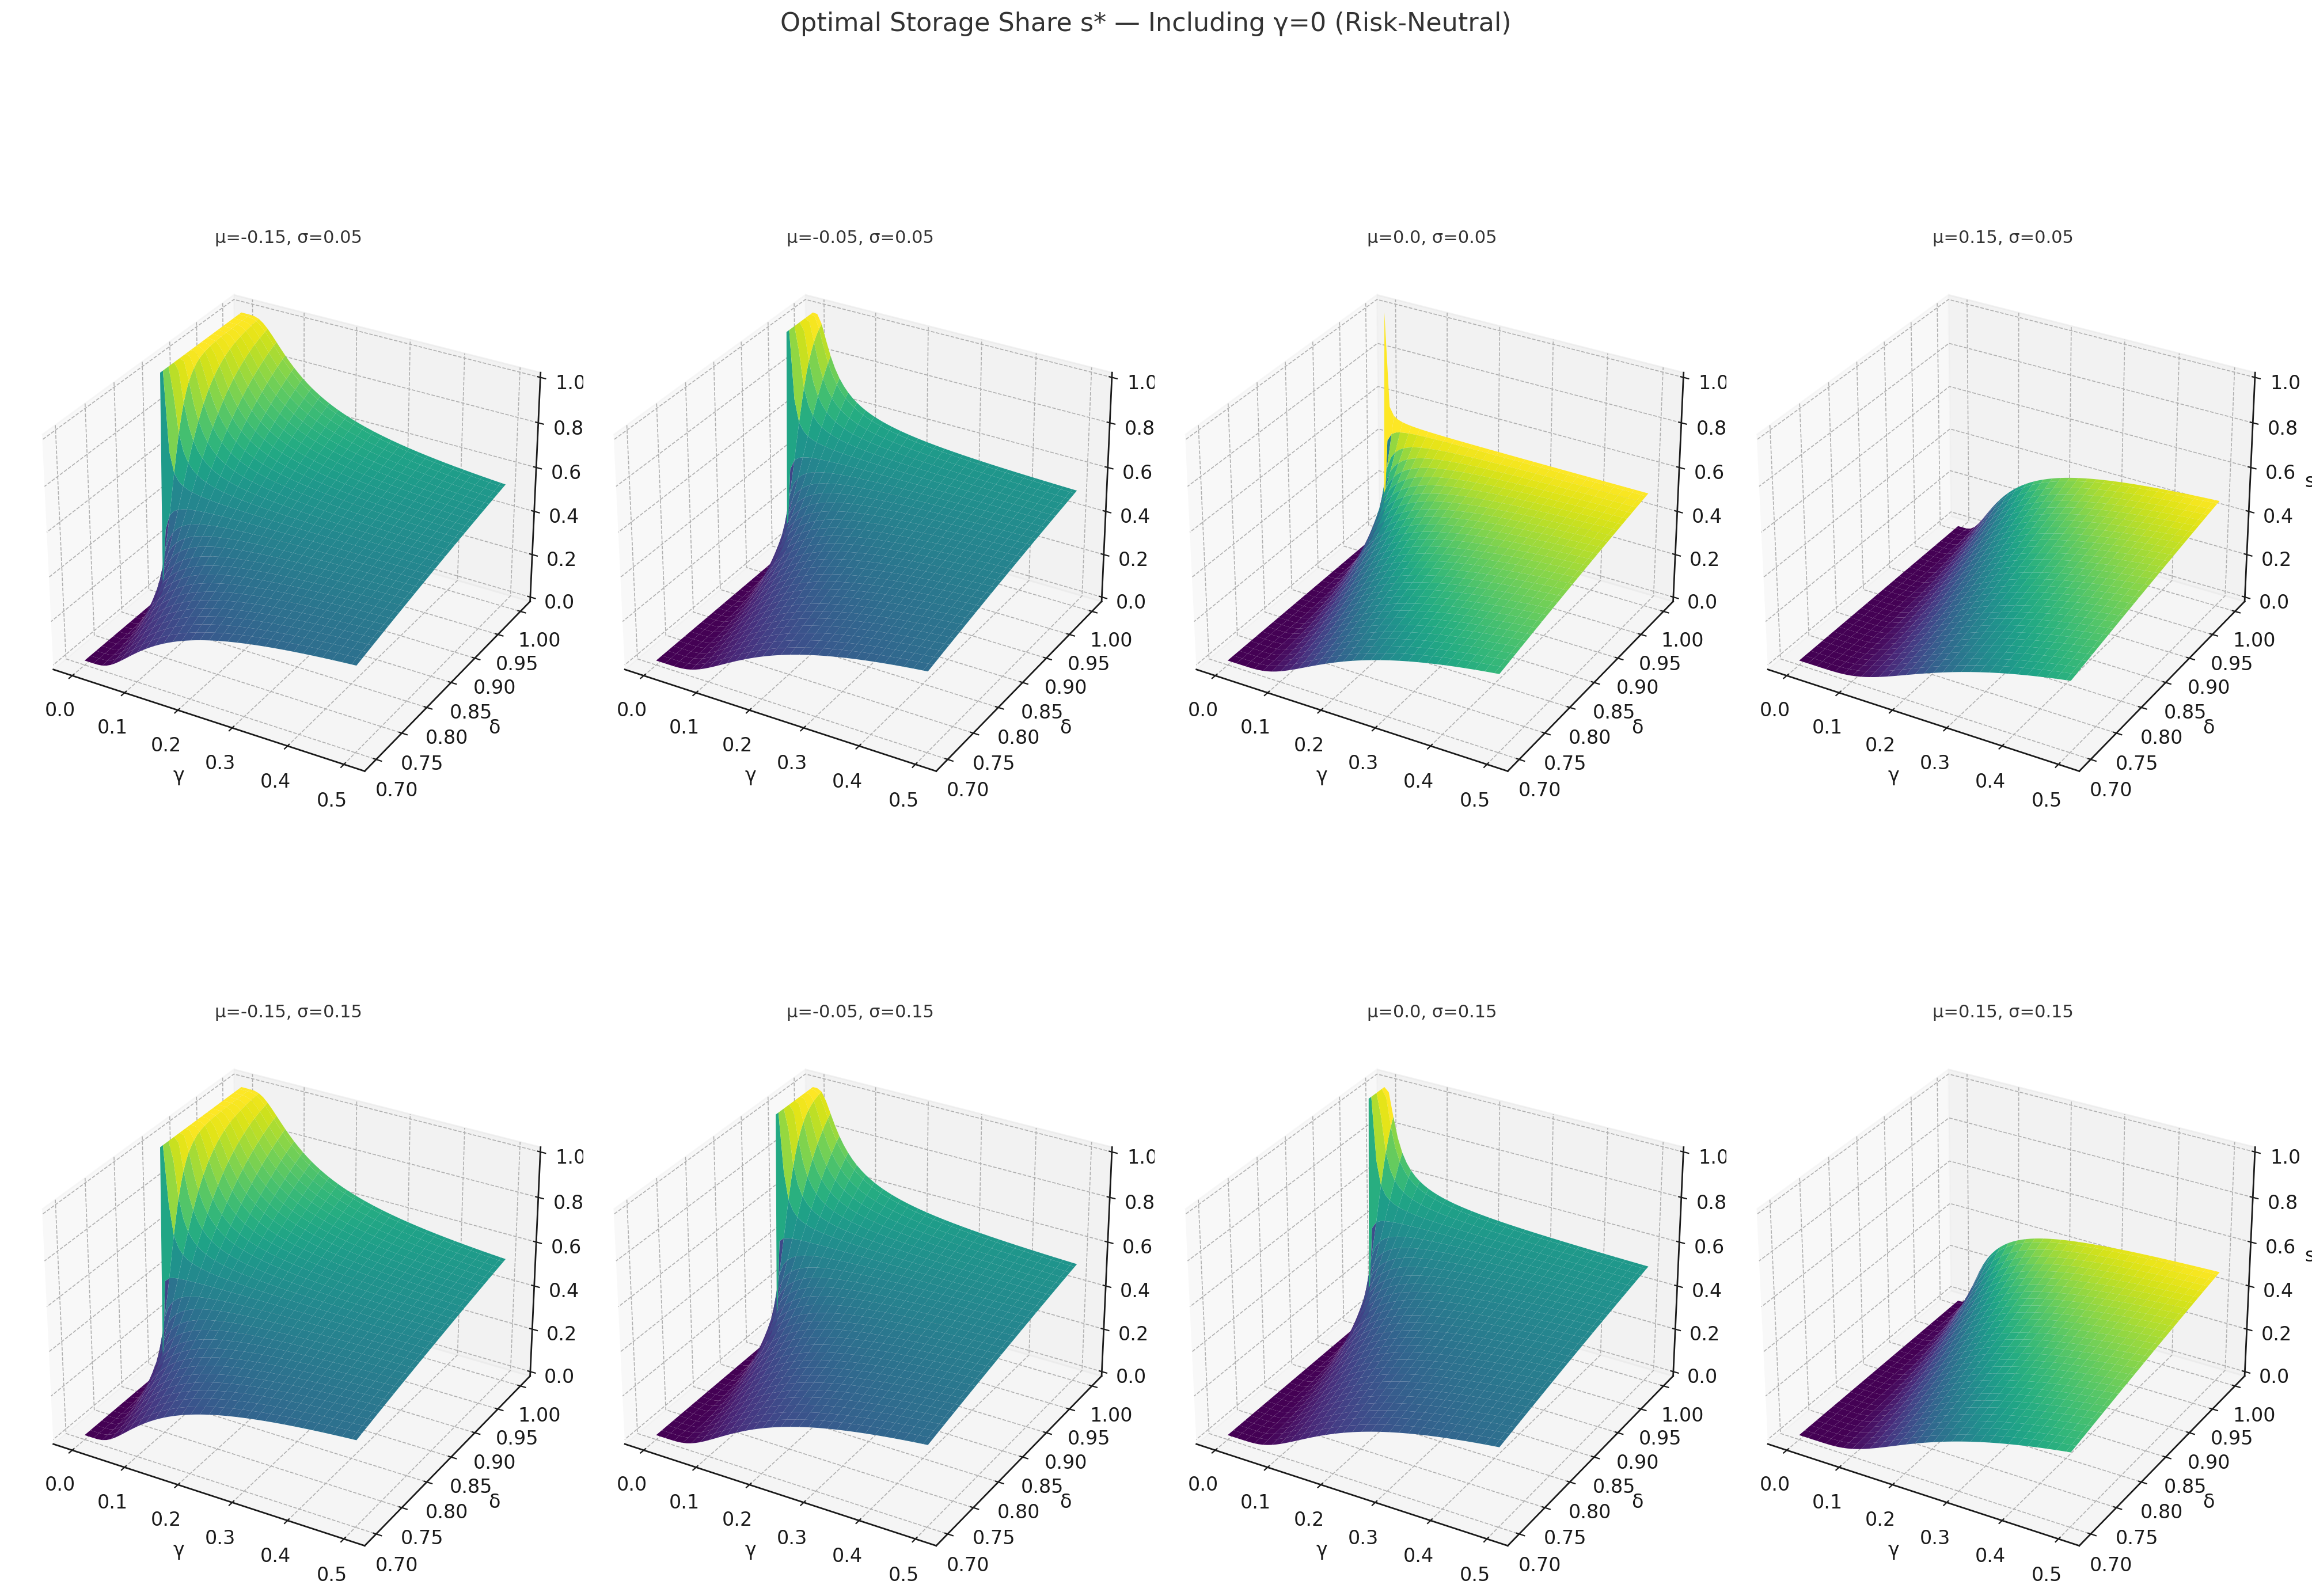
\includegraphics[width=\textwidth]{figures/first_p_0.5_s_optimal.png}
\caption{Optimal Storage Share 3D Visualizations}
\label{Figure: 3D optimal storage share}
\end{figure}


In general, a negative $\mu$ implies a decline in buyer power over time, leading to higher expected second-period prices and increased storage. Conversely, a positive $\mu$ (increasing buyer power) discourages storage. 

Higher variance $\sigma$ increases uncertainty. For risk-neutral farmers, this has no effect. But for risk-averse farmers, greater uncertainty reduces the appeal of storing due to the risk of low future prices.


\subsubsection{Sensitivity Analysis}
\noindent Building on the 3D visualizations constructed, I now conduct a focused sensitivity analysis to further dissect how optimal storage decisions respond to variations in farmers' discount factors, perceptions about future buyer power, and observed harvest prices.

Under the same assumption on the distribution of inter-temporal buyer power change, I examine three different risk aversion levels specifically: $\gamma = 0.05$ (very mild), $\gamma = 0.1$ (mild), and $\gamma = 0.35$ (moderate). For each $\gamma$, I first simulate how the optimal storage share varies along three dimensions separately:
\begin{itemize}
    \item The discount factor $\delta \in [0.7, 1]$,
    \item The standard deviation $\sigma_a \in [0.01, 0.20]$ of buyer power shocks,
    \item The observed first-period price $p_1 \in [0.6, 1.0]$.
\end{itemize}
Simulations are conducted for two beliefs about future buyer power: $\mu_a = -0.15$ (optimistic) and $\mu_a = 0.15$ (pessimistic).

Then, I also simulate how the move of the mean change in buyer power across two periods, $\mu_a \in [-0.25, +0.25]$, shapes farmers' optimal storage share. 

For each setting, I draw 200,000 Monte Carlo samples of $a$, compute the expectation term in Eq~\ref{Eq: optimal storage share, in form of kappa}, and solve for the interior optimal storage share. Simulations assume base values $p_1 = 0.8$, $\delta = 0.9$, and $\sigma_a = 0.10$ when not varying the dimension in question.


\begin{figure}[pht]
\centering
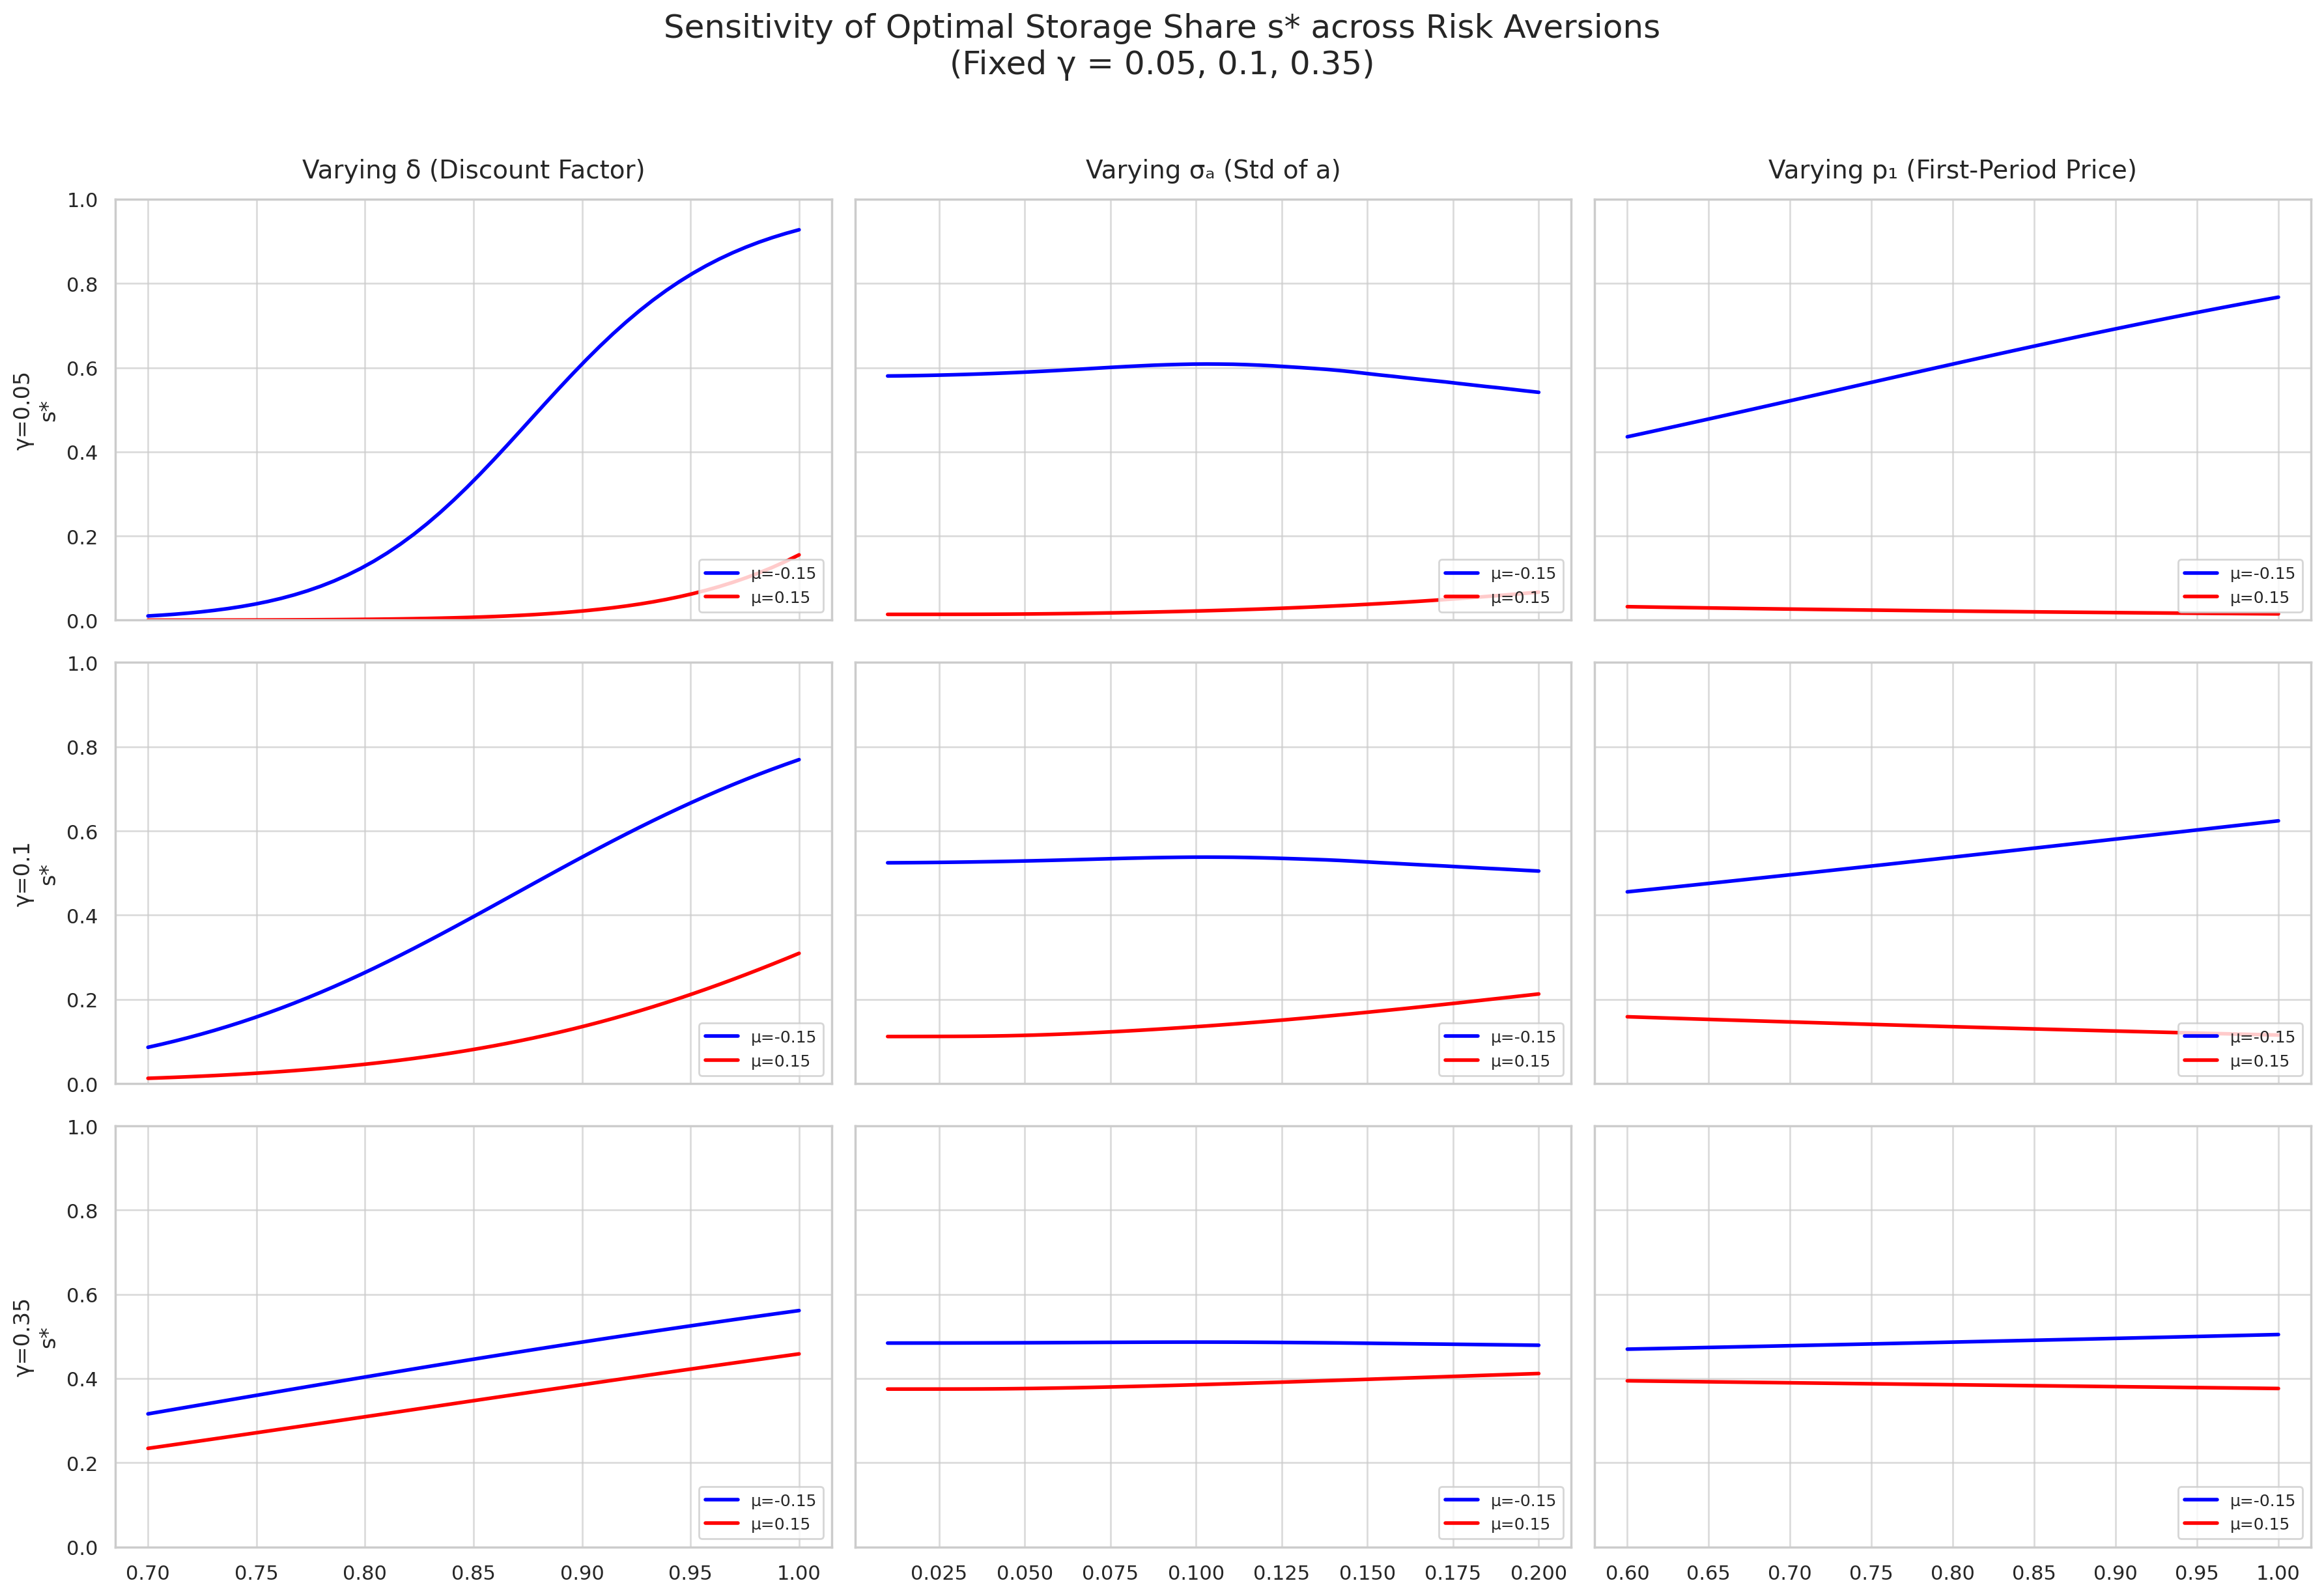
\includegraphics[width=\textwidth]{figures/sensitivity_comparative.png}
\caption{Comparative Sensitivity of Storage Decisions Across Risk Aversion Levels}
\label{Figure: sensitivity_comparative}
\end{figure}


The slicing exercises shown in Figure~\ref{Figure: sensitivity_comparative} reveal consistent and economically intuitive patterns, complementing the general trends observed in the 3D graphs.

First, \textbf{variation in the discount factor} $\delta$ strongly drives storage behavior across all $\gamma$. As $\delta$ increases (farmers become more patient or lower storage cost), the optimal storage share rises monotonically. The magnitude of this effect is larger when the farmer holds optimistic beliefs ($\mu_a = -0.15$) and when risk aversion is lower. As $\gamma$ increases, the storage gap between optimistic and pessimistic farmers widens substantially.

Second, \textbf{variation in the standard deviation} $\sigma_a$ of buyer power shocks highlights the role of risk aversion. At $\gamma=0.05$ and $\gamma=0.1$, uncertainty has negligible effects on storage. However, at $\gamma=0.35$, storage declines sharply with higher $\sigma_a$, particularly under pessimistic beliefs. This aligns with precautionary behavior in the presence of uncertainty.

Third, \textbf{variation in the observed first-period price} $p_1$ has a clear impact. Higher $p_1$ discourages storage, as selling immediately becomes more attractive. This effect is modest at low $\gamma$ but becomes stronger with higher risk aversion, especially when combined with pessimistic expectations.

\begin{table}[h!]
\centering
\begin{tabular}{lccc}
\toprule
Dimension Varied & Low $\gamma=0.05$ & Mild $\gamma=0.1$ & Moderate $\gamma=0.35$ \\
\midrule
Discount factor $\delta$ $\uparrow$ & $s^*$ rises moderately & $s^*$ rises strongly & $s^*$ rises very strongly \\
Std deviation $\sigma_a$ $\uparrow$ & negligible effect & small negative effect & sharp decline in $s^*$ \\
Observed price $p_1$ $\uparrow$ & $s^*$ falls modestly & $s^*$ falls clearly & steep fall in $s^*$ \\
\bottomrule
\end{tabular}
\caption{Comparative sensitivity of optimal storage share $s^*$ across risk aversion levels.}
\end{table}

\begin{figure}[htbp]
    \centering
    \begin{subfigure}[b]{0.45\textwidth}
        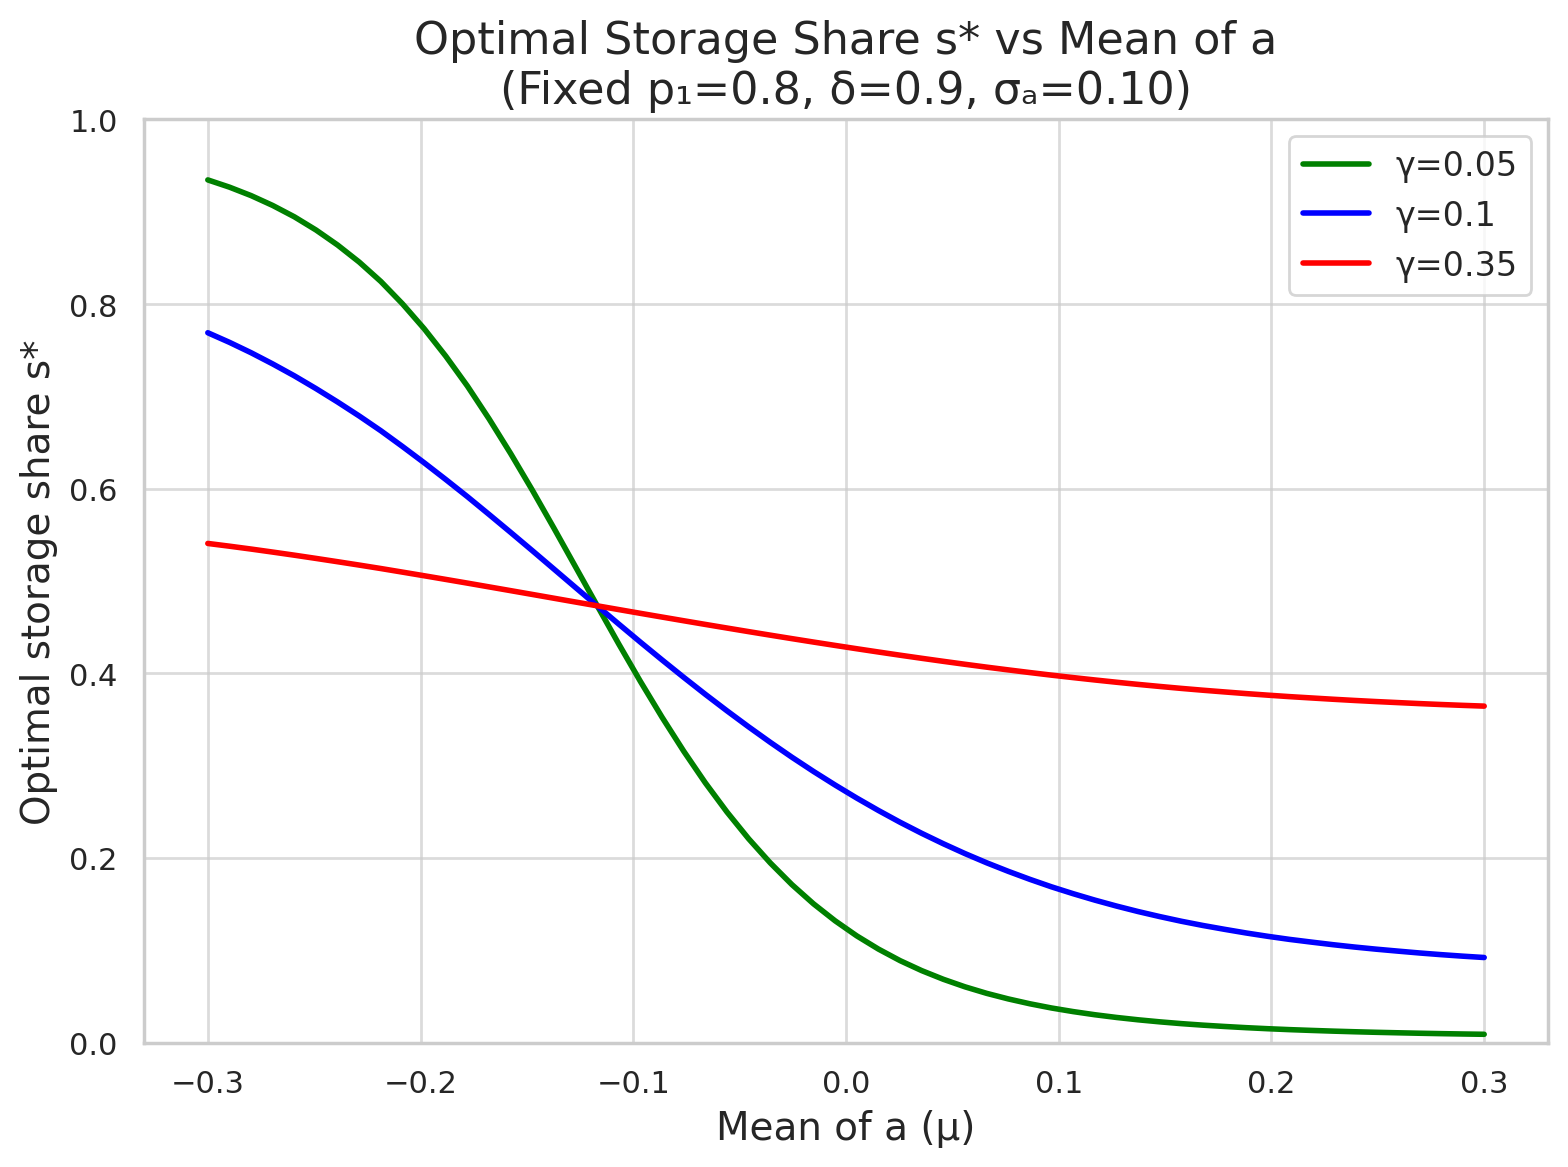
\includegraphics[width=\textwidth]{figures/storage_share_buyer_power_simulation.png}
        \caption{Future Market Expectations on Storage Behavior Across Risk Aversion}
        \label{fig: buyer power and optimal storage}
    \end{subfigure}
    \hspace{0.05\textwidth}
    \begin{subfigure}[b]{0.45\textwidth}
        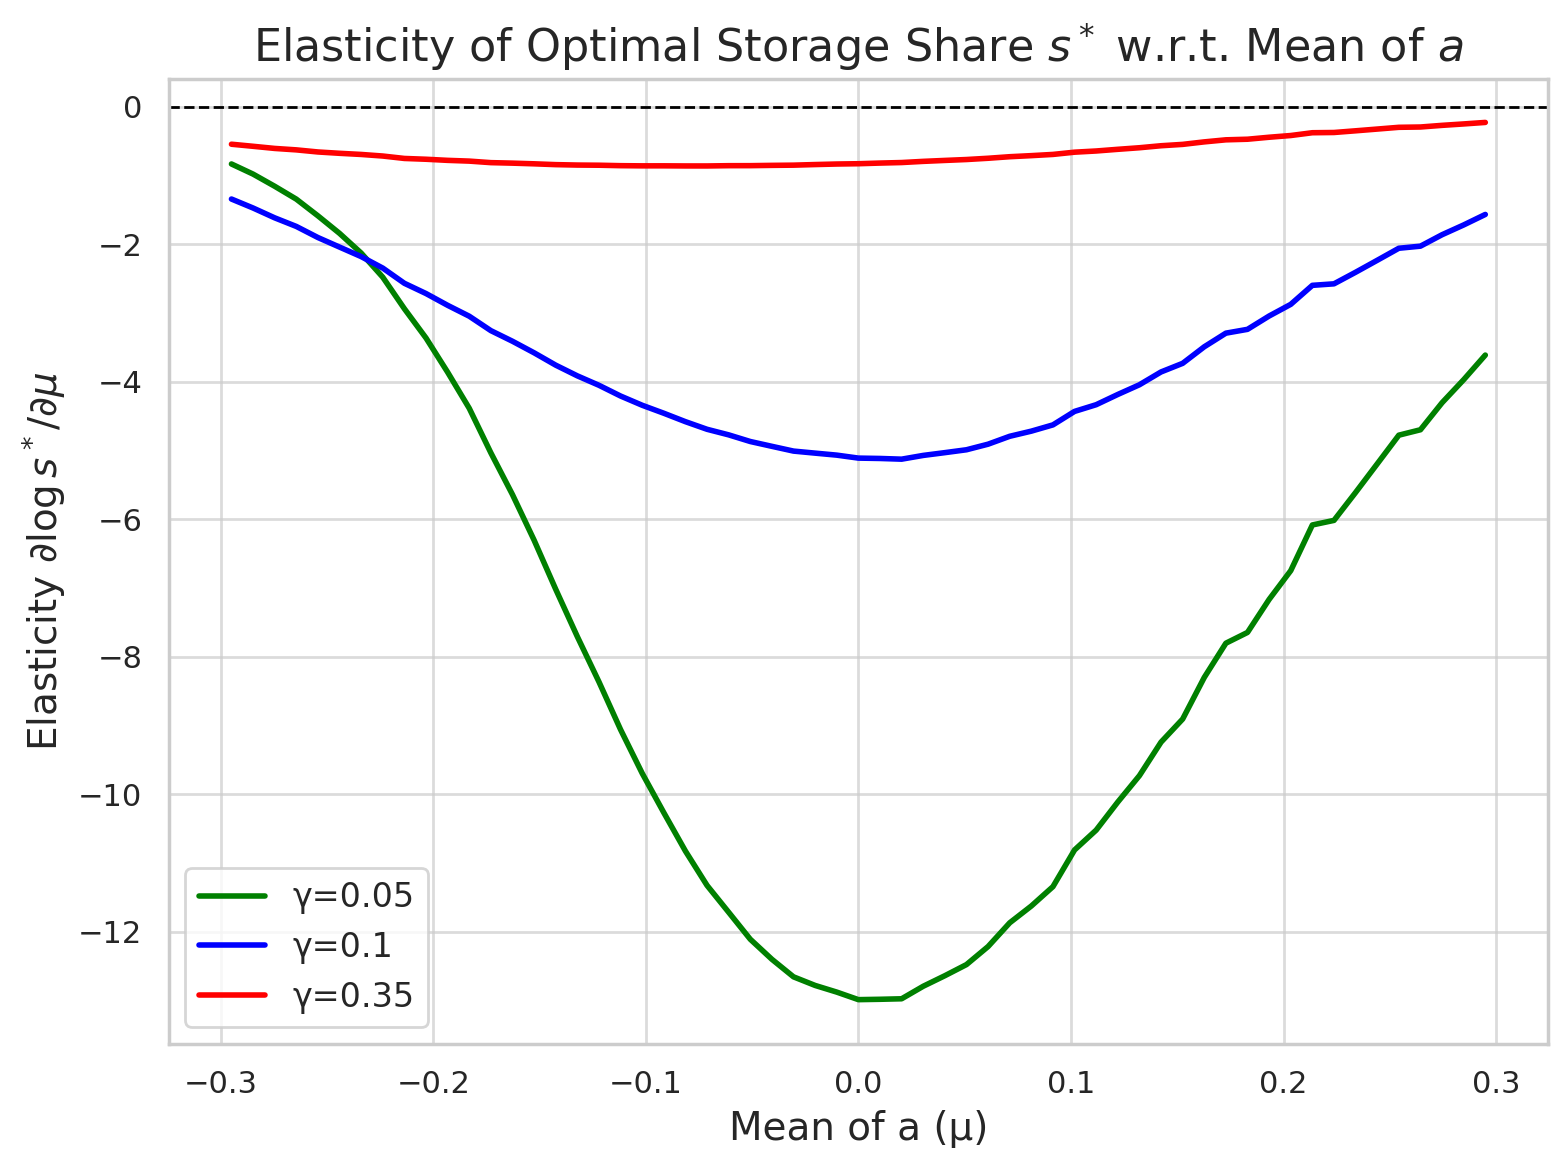
\includegraphics[width=\textwidth]{figures/elasticity_storage_buyer_power.png}
        \caption{Elasticity of Storage Decisions to Expected Market Conditions}
        \label{fig:elasticity of storage share to expected market conditions}
    \end{subfigure}
    \caption{Optimal Storage Share and Mean Buyer Power Change}
    \label{fig:wholefig}
\end{figure}


More importantly, as farmers' risk preference moves closer to risk neutrality, their storage decision tends to be more polarized. The left figure~\ref{fig: buyer power and optimal storage} below plots the optimal storage share $s^*$ against the mean of buyer-power changes $\mu$, holding constant the first-period price ($p_1 = 0.8$), the discount factor ($\delta = 0.9$), and the standard deviation of shocks ($\sigma_a = 0.10$). Across all three levels of risk aversion ($\gamma = 0.05$, $0.10$, and $0.35$), the storage share $s^*$ increases monotonically as $\mu$ becomes more negative---that is, as farmers expect buyer power to fall and future prices to improve. Farmers with very low risk aversion ($\gamma = 0.05$) exhibit consistently higher storage shares compared to those with moderate risk aversion ($\gamma = 0.35$), indicating that greater risk aversion significantly discourages storage. Near $\mu = 0$, small changes in beliefs have pronounced effects on behavior: a slight shift toward optimism (more negative $\mu$) substantially raises storage, while a slight shift toward pessimism (positive $\mu$) sharply reduces it. These patterns suggest that farmers' willingness to store is highly sensitive to expectations about future market power, particularly when their beliefs are close to neutral (expecting no temporal change in buyer power).

The right one, figure~\ref{fig:elasticity of storage share to expected market conditions} quantifies this sensitivity more precisely by plotting the elasticity of the storage share with respect to $\mu$, measured as $\partial \log s^* / \partial \mu$. Consistent with the storage patterns, the elasticity is negative throughout, implying that an increase in expected buyer power (worsening market conditions) leads to a reduction in storage. For farmers with very low risk aversion ($\gamma = 0.05$), elasticities are extremely large in magnitude (around $-13$) near $\mu = 0$, revealing an almost hyper-sensitive response to small changes in belief. As risk aversion increases ($\gamma = 0.35$), the magnitude of elasticity shrinks considerably (to about $-0.86$), indicating a dampened but still directionally consistent response. The elasticities peak in absolute value around $\mu \approx 0$ for all risk profiles, further highlighting that belief fragility is most pronounced when farmers perceive market conditions as roughly balanced between better and worse outcomes. Notably, there is no sign reversal in elasticity across the range of $\mu$; expectations consistently affect storage in the same direction.

Overall, these simulations confirm that the optimal storage share is highly elastic to both discounting and first-period price realizations, moderately elastic to beliefs about future buyer power, and increasingly sensitive to uncertainty as risk aversion rises.












\section{Extension: Explicit Competition Forms}
\noindent In the baseline framework above, buyer power is represented in a reduced-form manner through a nonlinear transformation into farm-gate prices. Specifically, buyer power $\theta$ was treated as an abstract, latent variable inferred from observed prices. To move beyond this abstraction, I now introduce explicit models of buyer competition. Suppose that instead of perceiving an unobservable level of buyer power, farmers observe the number of buyers $N$ present in the village at the time of harvest, and form expectations over future changes in $N$.


\subsection{Cournot Competition}
\noindent Under Cournot competition, each buyer chooses the quantity to purchase simultaneously, assuming that other buyers’ quantities are fixed. The resulting equilibrium reflects strategic quantity-setting behavior. In this setup, buyer power can be directly related to the number of buyers via $\theta = \frac{1}{N}$, where $N$ denotes the number of active buyers in a given period.

Given this relationship, and maintaining the same linear demand structure used in Section~\ref{Section: Middlemen Market Structure and Farm-Gate Price Formation}, the resulting equilibrium price in each period $t$ is:
\begin{equation}
    p_t = \frac{N_t}{N_t + 1}, \quad t = 1,2.
\end{equation}
\noindent This expression captures the inverse relation between market concentration and farm-gate prices: as $N_t$ increases, buyer power declines, and the price approaches the competitive limit of 1. Conversely, when $N_t$ is small, market power is significant, and prices are suppressed.



\subsection{Bertrand Competition}
\noindent In contrast, under Bertrand competition, buyers set prices rather than quantities. If there are no capacity constraints, standard Bertrand logic implies that even two buyers suffice to drive prices down to marginal cost. This phenomenon, known as the Bertrand Paradox, predicts perfectly competitive outcomes as long as $N \geq 2$.

Therefore, under Bertrand conditions, the farm-gate price received by farmers can be modeled as:
\begin{equation}
p_t = 
\begin{cases}
\underline{p}, & N_t = 1 \\
1, & N_t \geq 2
\end{cases},
\end{equation}
\noindent where $\underline{p} < 1$ denotes the monopsonistic reservation price paid when only one buyer is present. The transition from a single-buyer market to a multi-buyer market results in a discontinuous shift in price, characteristic of Bertrand dynamics.

\subsection{Implications for Market Characterization}

\noindent These two canonical forms of competition serve as polar cases. In practice, actual procurement market conduct may lie somewhere between Cournot and Bertrand. Collusion among buyers, capacity constraints, product differentiation, and repeated interactions could all prevent the realization of Bertrand outcomes, even in settings with multiple traders.

Rather than committing to either structure as a definitive description, I use them as bounding cases to characterize the range of possible outcomes. Cournot competition offers a smooth, parametric relationship between buyer numbers and prices, useful for comparative statics and policy simulations. Bertrand competition, on the other hand, highlights the potential for abrupt changes in pricing behavior with marginal increases in buyer participation.

Exploring these stylized models allows for deeper insight into how the structure of rural trading networks influences farm-gate prices. In subsequent sections, I assess how changes in $N$—either through policy interventions (e.g., reducing entry barriers) or stochastic shocks—translate into shifts in storage behavior and welfare outcomes for farmers.





% So, e.g., you could conduct a simulation with N = 2 at harvest and consider the storage decision for N = 3, 4, 5 in period 2.




% The framework shows that, absent an opportunity to observe more "draws" of the buyer-side competitive conditions, farmers would always sell during the first post-harvest period and avoid carrying costs or quality deterioration.

% The time-varying oligopsony power of middlemen is captured by assuming the existence of independent simplified Bertrand competition in each trading period, which allows a potentially higher farm-gate price to sell in future periods if a farmer chooses to store. I assume that there are only two traders in the market area, they compete with each other to purchase the crop from the growers, but each trader cannot visit every producing location, and hence $n \in\{1,2\}$, the number of traders at a specific village, is assumed to be stochastic in each trading period.\footnote{One possible explanation is the trader's limited resources, such as an insufficient number of trucks to visit every village. Another factor could be collusion among traders, leading to the allocation of markets, turning each trader into a monopsony in their assigned markets during the designated periods \citep{herings2005intertemporal}. However, collusion is prone to breakdowns, as cartels are inherently unstable. Therefore, even if trader collusion occurs in period 1, it may not persist into period 2.}\textsuperscript{,}\footnote{In the case of Bertrand competition, the inclusion of additional traders does not significantly impact the model. This is because, under Bertrand competition, the crucial determinant of equilibrium prices is whether only one trader or more than one trader visits. Having two traders is sufficient to yield a competitive outcome.}




%----------------------------------------------------%
%----------------------------------------------------%


\section{Further Extensions}

\subsection{Risk Aversion}
\noindent According to \cite{o2018modeling}, "Real-world risk aversion is clearly not as straightforward as expected utility suggests. Additional sources of risk aversion (or risk-seeking) need to be used instead of, or in conjunction with, diminishing marginal utility of wealth." Individuals assess options involving both gains and losses, the "kink" in the value function between losses and gains induces risk aversion. Therefore, future researchers may extend my model by exploring simple mean-variance or the Loss Aversion model \citep{kahneman1979prospect}, rather than the expected utility.

The approach developed by \cite{kHoszegi2006model, kHoszegi2007reference, kHoszegi2009reference} in addressing loss aversion with an endogenous reference point aims to mitigate this degree of freedom by asserting that the reference point is entirely determined by one's expectations about outcomes. Despite this, there has been limited progress in adapting alternative models to dynamic settings, with a notable exception of \cite{kHoszegi2009reference}, who define loss aversion concerning changes in beliefs regarding both current and future consumption.



\subsection{Collective-Action Dilemma: Storage "Treadmill"}
\noindent Another important observation from the fieldwork is that increasing storage adoption among farmers in a village would discourage traders from visiting there. If the majority of farmers in a village adopt storage, middlemen may redirect their focus to other villages where farmers have not yet embraced this technology. This spillover effect could stem from middlemen favoring farmers with less bargaining power, as they could negotiate lower prices for the crops they purchase. This leaves farmers without storage in this well-equipped village facing less competitive market conditions and creates in essence an escalating incentive within the village to obtain storage. However, the higher the adoption rate in this village, the lower the marginal benefit of storage adoption is as the less likely the traders would visit there. Therefore, this creates a storage "treadmill" similar to the technology treadmill envisioned by Willard Cochrane \citep{levins1996treadmill, cochrane1958farm}. Further analysis could discuss this collective-action dilemma and try to introduce a parameter into the current model to capture it.


\subsection{Non-linear Storage Cost}
\noindent Storage costs for farmers, defined as the sum of the actual cost of renting or operating storage space and the cost of deterioration, could be non-linear in many cases. For perishable goods like apples, the primary reason for convex storage costs is probably that spoilage and quality deterioration increase over time. Also, the operating costs of storage may not increase linearly with the volume of goods stored. Managing temperature and humidity conditions for larger quantities might require more sophisticated technology and energy consumption, leading to non-linear cost increases.

Supporting this notion, \cite{williams1989economic} demonstrates, through a quadratic form of total marketing costs, that farmers need to weigh the marginal revenue of later sales against the elevated costs incurred. This balance leads to a positive inventory, even without considering risk aversion. Instead of capturing the composite storage cost by a discounting factor, a well-designed mathematical model would allow other forms of storage costs, therefore, may give us other relevant real-world policy implications.



\section{Conclusion}
\noindent This chapter demonstrates that storage adoption can have a dynamic impact on the welfare of farmers facing oligopsony power, providing inter-temporal arbitrage opportunities and stronger bargaining power over time. Cold storage adoption, especially for storable crops, helps farmers overcome trading-time limitations and benefit even from temporal changes in trader competition alone. Examining storage from a market competition perspective offers a fresh approach to analyzing the influence of inventory on growers' and sellers' marketing strategies and their bargaining power.

My baseline model provides a theoretical basis for small-scale farmers' storage and marketing choices in developing countries. It focuses on farmers' intra-seasonal strategies and the storing-decision process, where farmers observe farm-gate prices at harvest and decide whether to immediately sell some, all, or none of their crops. When farmers have insufficient bargaining power at a single point in time, the adoption of storage at lower storage costs would give them inter-temporal arbitrage opportunities. 

Therefore, in many developing countries, future government policies can replace or supplement the existing minimum purchase price and direct cash transfers by subsidizing farmers' investment in storage infrastructure. Instead of intervening directly in markets, by using on-farm technology broadly to sell their harvest at an optimal time, the government can empower weak farmers to gain stronger bargaining power against middlemen and benefit both consumers and growers in the agricultural industry supply chains.

This chapter's application extends beyond the fresh apple industry to various settings. Cold storage and inventory play a crucial role in transactions, commonly seen as tools to help sellers take advantage of business cycle fluctuations. However, the competitive dynamics among buyers can vary over time, even without changes in demand or supply elsewhere in the industry chain. By examining storage from a market competition perspective, this model offers a fresh approach to analyzing the influence of inventory on growers' and sellers' marketing strategies and their bargaining powers in agricultural commodity industries.


\section{Rich's Feedback (Unsolved ones)}
\begin{itemize}
    \item Discuss fixed costs of storage (including costs of transporting product to a storage facility) as a factor that probably leads farmers to choose all or nothing vs. interior solutions to storage.
    
    \item I think you are OK subsuming storage costs as part of your delta, so delta represents a discount factor + storage costs. I don’t love this idea, but it simplifies things. Another way is to simply think of $P_2$ as being the price NET of a per-unit storage charge. Thus the farmer forms expectations of the future price based on an assessment of future market competition and then the net price he expects to realize is $E[P_{net}] = E[P_2(\theta)] - c$, where $c$ is the per-unit storage cost, which is known and not stochastic.
\end{itemize}